\chapter{介绍}
近年来,在人工智能领域,强化学习得到了极为广泛的重视和研究。强化学习是一种常见的人工智能范式,旨在解决智能体和环境交互中的决策问题。在这篇论文中,我们为解决一类特殊的问题(``稀疏奖励问题'')而提出了一种分层强化学习的架构。我们提出了一个新的分层强化学习算法``基于优势函数辅助奖励的分层强化学习''(Hierarchical reinforcement learning with Advantage-based Auxilliary Reward, HAAR),在强化学习社区常用的基准实验环境(Benchmark\cite{benchmarking_RL})中进行了实验测试,在相同的实验环境下与其他算法对比,取得了当前学术界的最佳成绩。在此基础上,我们把这套算法应用于自动驾驶仿真环境,解决了一个自动驾驶路径和速度规划的问题。

接下来,我们将会首先介绍强化学习的一般问题,其中将重点介绍分层强化学习这一重要分支,并由此引出强化学习中有待研究的问题,指出我们具体研究的问题及其意义。

\section{强化学习预备知识}
  在强化学习的著作\textit{Reinforcement Learning An Introduction}\cite{Sutton_book}中,Sutton对强化学习的理论进行了详尽的讨论。在这里,我们对强化学习的发展做一个精炼的综述,并从契合课题的框架进行一些讨论。另外,我们还将详细讨论强化学习的一些最新进展和它们在本课题中的应用。
  \subsection{问题描述}
    Sutton在1988年首次提出强化学习问题的一般描述\cite{Sutton_problem_formulation}。诸如学习走路、学习下棋的一般性问题都可以归为强化学习的问题。强化学习问题的四个基本元素是:一个策略(policy),一个奖励函数(reward),一个价值函数(value function)和一个环境模型(model)。例如,自动驾驶问题中,智能体面对它观察到的一个周边车流的\textbf{环境},会给出一个输出,例如以某一加速度加速。在采取这一行动之后,智能体会得到一个\textbf{奖励}(可能有延迟),例如它到达了目的地,我们给它价值$100$的奖励。而如何决定加速度,就是我们想要智能体去学习的\textbf{策略}。在制定策略的过程中,智能体会去试图衡量目前所处状态的\textbf{价值}(价值函数),例如周围车辆非常拥堵,这个状态的价值就比较低,是我们希望避免进入的状态;而车前非常空旷则可能是我们赋予价值较高,希望进入的状态。\par
    在这里,我们将用一些研究者所默认的记号对我们的问题进行数学抽象。假设下标$t$表示任一时刻,而$S_t$代表某一时刻的状态,$A_t$表示智能体采取的行动,$\pi$表示智能体的策略,$R_t$表示智能体某一步获得的奖励。我们的目标是让智能体通过学习,获得尽可能大的总奖励,记为$G$。有时我们可以定义
      $$ G = \sum_{t} R_t $$
    但是多数时候我们会考虑加入一个折扣$\gamma$($0 < \gamma < 1$),认为一个行为直接获得的奖励对它更有意义,而很久以后获得的奖励与这个行为的关联越来越小,记为
      \begin{align}
        G_{t_0} = \sum_{t = t0}^{t_n} \gamma^{t-t_0} R_t
        \label{eq:G}
      \end{align}
    \par 其中$t_n$要么是一个过程因为某种原因终止的时刻,要么是$\infty$
    \par
    强化学习解决的是一个马尔可夫决策过程(MDP)\cite{Bellman_MDP}。在MDP中,$S_{t+1}$只取决于$S_t$和$A_t$,而不受到之前历史过程的影响。也就是说,$S_t$状态本身就包含了它所有的历史对后续过程的影响。在这个假设下,我们可以这样表达强化学习的目标\cite{DRL_for_driving}:记$v^{\pi}(s)$为状态$s$的价值函数。我们有$$ v^{\pi}(s) = E[G_{t_0} | S_{t_0} = s, \pi(s) ] $$
      $$ J(\pi) = \max_{\pi} E(v^{\pi}(s)) $$
      $$ \pi^*(s) = \argmax_{\pi} J(\pi) $$
    \par 强化学习的终极目标就是找到这个$\pi^*(s)$。Bellman在\textit{Dynamic Programming}一书中提出了著名的Bellman最优性等式\cite{Bellman_DP}
    \begin{align}
       v_*(s) = \max_{a} \sum_{s', r}p(s', r | s, a)[r + \gamma v_*(s')]
    \end{align}
    \par 同时,我们用$q(s, a)$表示在状态$s$下采取行动$a$可以获得的价值,那么Bellman最优性等式又可以表示为
    \begin{align}
       q_*(s, a) = \sum_{s', r}p(s', r | s, a)[r + \gamma \max_{a'} q_*(s', a')]
    \end{align}

    \par 这两个表达式在后续的推导中会非常有用。
    
  \subsection{强化学习典型算法综述}
      强化学习包含许多的算法,也有很多分类方法。其中,有一大类是列表方法,可以理解为是把$v(s)$保存起来的方法;另一大类是近似方法,也就是用一个函数去近似$v(s)$\cite{Sutton_book}。其中,第二类方法在近年来使用最多,神经网络使得函数可以近似非常复杂的映射关系,也让许多复杂问题通过强化学习得到了解决。\par
      列表式的强化学习方法包括动态规划\cite{Bellman_DP},蒙特卡罗方法,时序差分学习(Temporal-difference learning,简称TD方法,包括Sarsa\cite{Sutton_book}, Q-learning\cite{Q_learning})\cite{Sutton_problem_formulation},多步自助法\cite{n_step_bootstrapping}(n-step bootstrapping),Dyna规划方法\cite{Sutton_book}等。\par
      TD方法是列表法强化学习的核心。这一族的算法有许多衍生版本,但其核心是利用经验不断更新价值函数$V(s)$,直至其收敛。更新的基本模式为
      $$ V(s) \gets V(s) + \alpha [r + V(s') - V(s)] $$
      \par 其中,$\alpha$表示函数更新的步幅。而当我们用$Q(s, a)$去替代$V(s)$的时候,算法就成为了Sarsa(state, action, reward, state, action \cite{deepRL_overview}):
      $$ Q(s, a) \gets Q(s, a) + \alpha [r + \gamma Q(s', a') - Q(s, a)] $$
      \par 注意这里,$a'$是依据当前策略$\pi$采取的行动。而当我们把$Q(s', a')$替换成$\max_{a'} Q(s', a')$的时候,算法就成为了Q-学习法(Q-learning):
      \begin{align}
      \label{eq:Q_learning}
        Q(s, a) \gets Q(s, a) + \alpha [r + \gamma \max_{a'} Q(s', a') - Q(s, a)]
      \end{align}
      \par 在这里,我们发现Sarsa和Q-学习的重要区别:Sarsa是同策略学习的(on-policy),估算$Q$值时采用的策略就是当前策略,而Q-学习是采用异策略(off-policy)学习的,估算$Q$值时采用的策略不是当前策略,而是最优策略。同策略与异策略也作为强化学习中的两种并行方法,本身并不改变算法架构,但是会影响收敛性等特性。许多算法都可以在这个维度上进行变异。\par
      注意到在以上的算法中,我们每一步都对$Q$或者$V$进行更新。在多步骤自助法(n-step bootstrapping)中,我们则将更新进行延迟。例如,某一行动结束,$n$步过后,我们才观察这一行为造成的影响,并且对它的值进行更新,其更新方式如下
      $$ V(S_t) \gets V(S_t) + \alpha(G_{t:t+n} - V(S_t)) $$
      \par 其中,$G_{t:t+n} = \sum_{i = 1}^{n}\gamma^{i-1}R_{t+i} + \gamma^n V(S_{t+n})$
      \par Sutton等人指出,多步骤自助法强化学习在训练时的表现往往比蒙特卡罗和TD方法都要更优\cite{Sutton_book}。
      \par 归功于深度强化学习的提出\cite{atari_2013}\cite{deepRL_overview},近似函数的方法在近年来得到了极大的发展。近似函数有两种基本思路。第一种,是用某一类型的函数去近似状态的价值函数$v(s)$,从而帮助智能体根据不同的$v$采取不同的策略。第二种思路是跳过$v$的计算,而直接使用函数去近似一个策略$\pi$。在第二种思路中,$\pi(s)$的输出将直接是智能体应该采取的行为(或者行为的一个概率分布)。这种方法被称为``策略优化'',围绕策略优化问题衍生出一系列的策略梯度求解方法,成为近年来强化学习的热点研究方向之一。进一步的,在策略优化问题中,如果我们同时对价值函数$v(s)$进行近似和更新,那么可以得到一类框架,我们称之为actor-critic架构\cite{Sutton_book}。在后续的篇目中,我们会对此进行具体介绍。\par
      在深度强化学习中,比较著名的算法有DDPG\cite{DDPG},A2C\cite{A3C},TRPO\cite{TRPO},ACKTR\cite{ACKTR},ACER\cite{ACER},PPO\cite{PPO}等。这些算法全部忽略了环境的模型,或者环境模型是学习得到的(TRPO)。还有一类算法,其中的环境模型是提前设计建模得到的而非习得,其中有代表性的就是AlphaZero\cite{AlphaZero}。这类算法也是我们想探究的方向——是否通过提前建模,能够让自动驾驶车辆在环岛这类复杂环境中有更好的表现?在接下来的章节中,我们会详细介绍其中有代表性,并且在我们的场景下易于使用的算法。\par
      另外,在对价值函数进行优化时(梯度下降),不同的算法可能带来不同的结果。A3C采用了RMSProp算法\cite{RMSProp},我们往往还可以选择随机梯度下降法(SGD),带动量的随机梯度下降法\cite{SGD_momentum}等方法,在算法设计时需要进行尝试和选择。Sutton在书中对此进行了讨论\cite{Sutton_book}。此外,Ruder在2016的一篇综述文中对各种梯度下降算法进行了详尽的探讨\cite{GD_overview}。
      
    \subsection{无模型的深度强化学习}
      无模型的深度强化学习是我们在本课题中的重要算法基础之一。其中,2017年被提出的TRPO算法\cite{TRPO}是我们在本课题中的重点。基于TRPO,我们构建了分层结构,并且基于TRPO中策略单调提升的结论,我们证明了HAR算法的单调性。因此接下来我们将介绍无模型的深度强化学习问题及其典型算法。
      
      Mnih等人在2013年首度提出深度Q-网络(deep Q-network,简称DQN)\cite{atari_2013},2015年,他们的另一篇论文同样描述了DQN\cite{nature2015},激发了一轮深度神经网络与强化学习结合的热潮\cite{deepRL_overview}。DQN的基本思路是创造一个很一般的端到端的网络$Q(s, a | \theta)$,其中$\theta$是这个网络的参数。例如对于一个游戏,网络的输入直接就是未处理的图像,输出直接就是在某个阶段,游戏中的动作对应的价值。在传统Q-learning的框架下,DQN在每一步更新$q(s, a)$值的时候,不是直接使用\eqref{eq:Q_learning},而是利用梯度下降法去更新网络$Q$的参数$\theta$,使得$Q$估值总损失最小
      \begin{align*}
        \bigtriangledown_{\theta_i}Loss(\theta_i) = E_{s, a, s'}[(r+\gamma \max_{a'}Q(s', a'|\theta_{i-1}) - Q(s, a|\theta_i))\bigtriangledown_{\theta_i}Q(s, a|\theta_i)]
      \end{align*}
      这里DQN的网络结构参考了Hinton等人提出的AlexNet\cite{AlexNet},也就是典型的卷积神经网络(CNN)结构。DQN的最大贡献在于,由于使用了经验回放的方法,DQN可以收敛,从而使得深度神经网络在强化学习中的应用成为了可能。由于神经网络的高度非线性,DQN得以模拟足够复杂的场景。DQN在Atari系列游戏中取得了突破性的进展,甚至在一些游戏中超越了人类专家的水平。\par
      不过由于我们想探究的问题更多地涉及到低维度的传感器信息输入,而不是高维度的图像直接输入,因此DQN一类的方法对我们的帮助并不是很大。而策略梯度方法则对我们有很大的借鉴意义,因此我们也将集中讨论这一类的方法。\par
      前面我们提到,在策略优化问题中,有一类架构被称为actor-critic架构。Mnih等人在2016年提出的A3C(asynchronous advantage actor-critic)算法\cite{A3C}成为应用actor-critic架构的经典案例。A3C算法同时维护一个策略函数$\pi(a|s; \theta)$和一个价值函数的估计$V(s; \theta_v )$,这两个函数均为卷积神经网络CNN,并且两个网络除了输出层以外的层均是共享的。其中, $\pi(a|s; \theta)$称为actor,而$V(s; \theta_v )$称为critic。actor-critic会计算一个``优势'',定义为$\delta = R + \gamma V(S'; \theta_v) - V(S; \theta_v)$\cite{Sutton_book}。A3C借鉴了多步骤自助法的思路(设步数为$k$),在计算优势时,变异为$\delta_t = \sum_{i = 0}^{k - 1}\gamma^i r_{t+i} + \gamma^k V(S_{t+k}; \theta_v) - V(S; \theta_v)$。每一步,我们依然对$\theta$和$\theta_v$进行更新,梯度的计算方法如下(注意计算梯度以后,还需要选择一个梯度下降方法对$\theta$和$\theta_v$进行更新)
      \begin{align}
      \label{eq:A3C_gradient1}
          d\theta &= \delta_t \bigtriangledown_{\theta} log_\pi(A_t|S_t; \theta)\\
      \label{eq:A3C_gradient2}
          d\theta_v &= \delta_t \bigtriangledown_{\theta_v} \delta_t^2
      \end{align}
      \par 如果我们采用多个智能体并行训练,把它们各自的梯度叠加在一起(也就是累加每个智能体各自求得的\eqref{eq:A3C_gradient1}\eqref{eq:A3C_gradient2}式),最后统一更新$\theta$和$\theta_v$,就称之为异步训练方法,这种算法也因此被称为asynchronous advantage actor-critic。如果条件受限没有异步,而只是用一个智能体进行训练,这个算法就称为A2C(advantage actor-critic)。actor-critic架构被认为是能够有效加速训练的,因此越来越多的算法都基于这一架构进行设计。\par
      2015年,Schulamn等人提出了经典的(Trust Region Policy Optimization, TRPO)算法\cite{TRPO}。在文章中,他们首先从理论上证明了一种策略迭代更新的MM(minorization-maximization)算法,可以确保策略对应的总价值($\eta(\pi) = E_{s_0}[\sum \gamma^t r(s_t); \pi_\theta]$)单调不下降。依据这一理论基础,他们进行了多步近似,将MM算法中的优化(求$\argmax$)的问题转化为了一个更简单的加限制的优化问题(信任空间优化,trust-region optimization)。在进行进一步近似后,优化式中的期望形式可以用蒙特卡罗方法进行估算。最后,优化式本身则利用一种近似的方法进行优化。在实验中,他们采用了神经网络作为策略$\pi$的表达。TRPO的更新方法是:
      \begin{align}
        \begin{aligned}
          \theta = \argmax_\theta E\bigg[\frac{\pi_\theta(a|s)}{\pi_{\theta_{old}}(a|s)}Q_{\theta_{old}}(s, a)\bigg]\\
          \text{subject to } E[D_{KL}(\pi_{\theta_{old}}(\cdot|s)||\pi_\theta(\cdot|s))] \leq \delta
        \end{aligned}
      \end{align}
      \par 其中,$\delta$是一个认为选定的小值。注意,在论文的附录中,作者提出采用一阶近似对上式进行求解,优化问题就可以就变为一个典型的拉格朗日共轭问题\cite{Convex_optimization_book}。不过,由于TRPO只是保证了每一步更新,策略都变得更好,却没有考虑探索性,因此,TRPO的结果很容易困在局部最优值。在Schulman之后,Wu等人于2017年又提出了一个改进算法ACKTR\cite{ACKTR}(Actor Critic using Kronecker-Factored Trust Region),采用actor-critic架构,并利用Kronecker因子去近似梯度下降。同年,Schulman等人又提出了PPO算法\cite{PPO},在实现难度和算法表现方面取得了平衡。PPO算法的基本思路有三点:
      \begin{itemize}
        \item 去除TRPO的优化限制条件,在TRPO的基础上,采用一个clip函数,从而阻止$\theta$每一次更新太大,确保收敛
        \item 在优化的函数里,通过引入系数的形式,同时优化actor和critic,整个优化过程只有一个优化目标函数
        \item 通过在优化目标中加入一个熵奖励,增加算法的探索性
      \end{itemize}
      \par PPO把强化学习问题转化为一个形式简单的单一函数优化问题,在许多方面取得了比以往算法(A2C, ACER, TRPO, etc.)更优的表现。\par
      在2015年,Silver首度提出了针对连续动作空间的确定性算法DPG(deterministic policy gradient)\cite{DPG}。与确定性算法对应的是随机算法,也就是策略是行动的概率分布。在高维的动作空间内(例如动作是连续的),DPG比与之对应的随机算法获得了更优的结果。DPG采用actor-critic架构,并且是异策略(off-policy)训练的。注意这里,DPG的actor-critic架构与Sutton书中提到的actor-critic架构有所区别。它是不以价值函数作为基准的,而正常的actor-critic架构应该以价值函数作为基准,计算优势,再进行求导\cite{Sutton_book},参见前面提到的A3C算法\cite{A3C}。同时,DPG算法采用的是Q-learning结构,不是用$V(s)$对价值进行估计,而是用$Q(s, \pi(s))$对价值进行估计。由于算法本身是确定性的,DPG与随机异策略actor-critic架构\cite{off-policy_actor-critic}不同,不需要针对策略进行重要性采样(importance sampling,在\cite{Sutton_book}中有详细讨论)。DPG本身没有选择神经网络,而是可以采用一般的函数,尤其是线性函数。\par
      DPG算法对$\pi(s)$和$\mu(s)$的更新方法如下:
      \begin{align}
        \begin{aligned}
          &\delta_t = r_t + \gamma Q(S_{t+1}, A_{t+1};\theta_Q) - Q(S_t, A_t;\theta_Q)\\
          &\theta_Q \gets \theta_Q + \alpha_{\theta_Q}\delta_t \bigtriangledown_{\theta_Q}Q(s, a;\theta_Q)\\
          &\theta_\mu \gets \theta_\mu + \alpha_{\theta_\mu}\bigtriangledown_{\theta_\mu}\mu(s;\theta_\mu)\bigtriangledown_{a}Q(s, a;\theta_Q)|_{a = \mu(s;\theta_\mu)}
        \end{aligned}
        \label{eq:DPG_update}
      \end{align}
      \par 基于DPG,Lillicrap等人提出的改进算法,DDPG算法\cite{DDPG},则全面采用了深度神经网络。为了能够让训练收敛,DDPG使用了一个目标网络(target network)的概念。目标网络的定义是缓慢地跟踪依据梯度下降优化得到的网络参数$\theta_Q$和$\theta_\mu$,$\theta_Q$是状态行动对的价值估计网络$Q$的参数,而$\theta_\mu$是actor-critic架构中actor采用的策略的参数。目标网络参数$\theta_Q'$和$\theta_\mu'$的更新方法如下(在每一步迭代过后进行这个更新):
      \begin{align*}
        \theta' = \tau \theta + (1-\tau) \theta', \tau \ll 1
        \label{eq:target_network}
      \end{align*}
      \par 这样,相当于强迫目标网络缓慢地变化,从而增强了训练的收敛性。目标网络主要用于带入\eqref{eq:DPG_update}中$\delta_t$的计算。同时,DDPG采用了经验回放的方法,在每一步迭代中都采用之前历史中一批随机挑选的过往经验进行批量计算,而非一步的结果,这样可以确保网络训练时不带有时序偏差。另外,DDPG没有像DPG一样采用异策略学习,而是在策略基础上加上一个噪声分布以确保``探索''性。\par
      
    \subsection{基于模型的强化学习}
    基于模型的强化学习并非本课题的重点,但是是强化学习问题当中重要的一部分,和无模型的强化学习算法并驾齐驱。目前,分层强化学习问题多数基于无模型的强化学习算法,很少考虑模型问题。但是实际上,模型可以大大提高算法的成功率、采样效率和稳定性。为完整性考量,在这里我们也对基于模型的强化学习算法进行简要的介绍,也作为给未来研究方向的一个灵感。
    
    基于模型的深度强化学习问题可以分为模型是``习得''的和模型是给定的两种。在这里,我们首先关注一下给定模型的强化学习的应用。
      \par 在模型给定的算法中,最著名的例子就是2016年提出的AlphaGo\cite{AlphaGo}。Deepmind在2017年进一步提出了AlphaZero\cite{AlphaZero},其算法和AlphaGo相比有几大特点:
      \begin{enumerate}
        \item AlphaZero完全采用逐步迭代的方式,而AlphaGo在训练中会挑选之前出现过的最好策略
        \item AlphaZero拥有的先验知识只有棋盘的格局和下棋的规则,并且这些知识只用来进行模拟
        \item AlphaZero对参数的变动更加鲁棒,不同棋类游戏用的都是同一套参数
        \item AlphaZero在训练中没有对输入进行任何数据加强的操作,而AlphaGo则对棋盘进行了镜像操作
      \end{enumerate}
      \par AlphaZero采用蒙特卡罗树状搜索(Monte Carlo Tree Search, MCTS\cite{Sutton_book})的方法,每次优先访问训练历史中访问次数低,但访问概率$\pi(a|s)$应该较高,且$Q(s, a)$的状态行为对$(s, a)$。同时,在此基础上加上一个噪声(在AlphaZero的例子中,一个狄利赫里分布的噪声),确保探索性。AlphaZero采用深度卷积神经网络作为策略$\pi(s)$的拟合函数,其输出为$\pi(s) = (\mathbf{p}, v)$,其中,$\mathbf{p}$为在某个状态下选择各个行为的概率,$v$为根据$s$推测的状态估值,$v = \mathbb{E}[z]$(胜负平局,$z$的值分别为$+1, -1, 0$)。针对该网络定义的损失函数为
      \begin{align}
        L = (z-v)^2 - \pi^T log \mathbf(p) + \lambda ||\theta||^2
      \end{align}
      \par 可以看出,这个损失函数试图使$v$的预测和棋局结果$z$更加接近;$\pi$代表了训练中各个动作的搜索概率,损失函数试图让神经网络的输出$\mathbf(p)$与之尽可能接近。
      \par 这里所谓“给定模型”,其实就是环境是已知的,不需要真的和环境交互,而是在仿真里直接进行下棋这个活动即可。然而,这也意味着这个问题本身与直接和未知环境交互并没有区别。尽管模型给定,算法并没有从模型本身得出什么规律,因此这个模型本质上就是一个环境。\par
      在强化学习问题中,从与环境的交互历史中逐渐学习到模型,则是另一个有趣的思路。在\cite{Sutton_book}中,Dyna架构就是这样一种思路。在强化学习中,利用模型去近似求解$v(s)$是一个``规划''(planning)问题。传统的列表式方法可以根据训练中得到的环境反馈不断更新模型。2015年,Oh等人在\cite{action-conditional_prediction}一文中提出了一种利用神经网络学习高维度环境的方法,使得复杂环境的模拟也成为了可能。\par 
      基于\cite{action-conditional_prediction}的结果,Racani\`{e}re等人在论文\cite{I2A}中提出了一种利用模型去增强无模型强化学习的方案,简称为I2C算法。这种方法本质上是细化了的A3C算法。注意到A3C本身是一个无模型的方法,它仅仅依赖于$\pi(a|s)$和$v(s)$的估计(回顾一下\eqref{eq:A3C_gradient1}\eqref{eq:A3C_gradient2}两个更新式)。但是,I2C算法修改了$\theta$的组织形式,构建了一个较为复杂的网络结构,因而引入了环境模型。其基本架构如图\ref{fig:I2A}所示。
      \begin{figure}[H] % use float package if you want it here
        \centering
        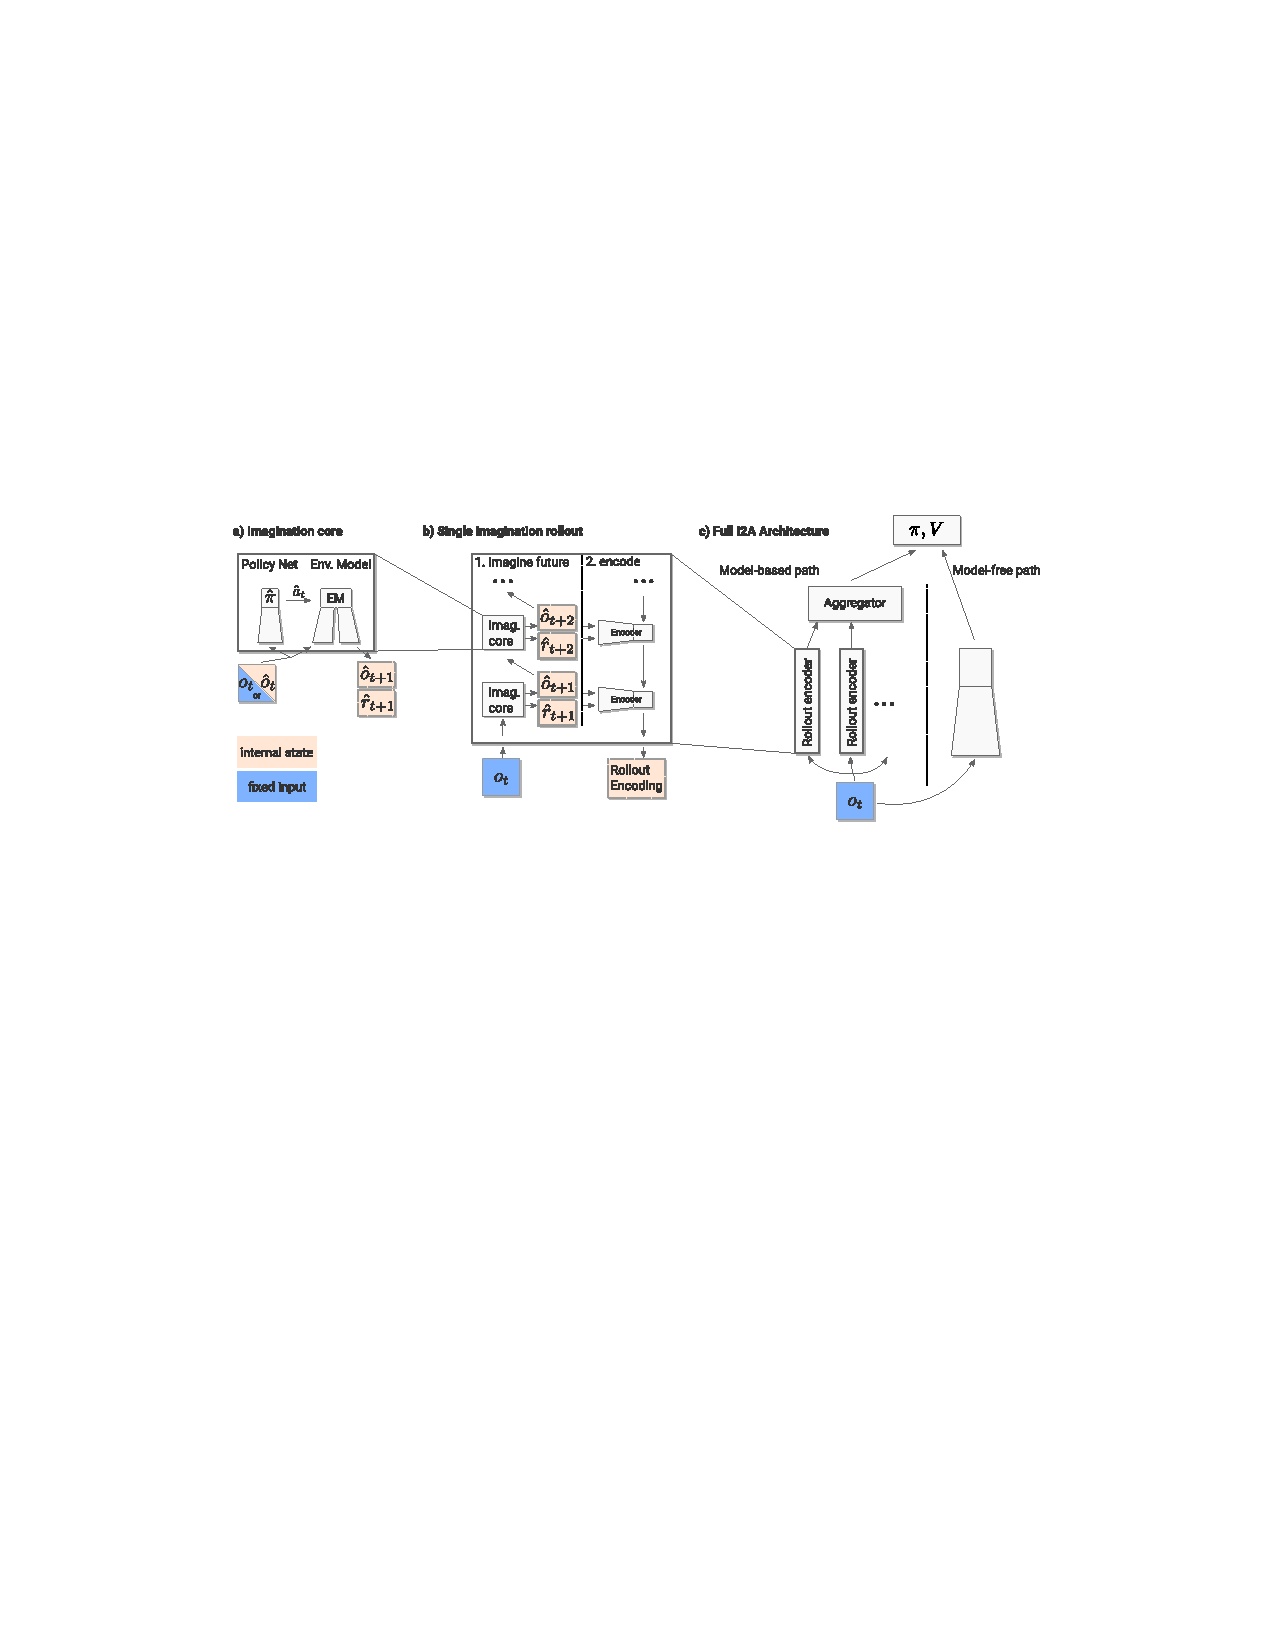
\includegraphics{I2A}
        \caption{I2A的基本结构:a) 一个预先训练好的神经网络,可以预测在策略$\hat{\pi}$下,状态$s$的一系列时序变化;b) 一个子网络,用于``理解''a)的输出结果;c) 整体架构}
        \label{fig:I2A}
      \end{figure}
      \par 图\ref{fig:I2A}c)展示了网络整体架构,可以看到整体网络的输入为$o_t$,也就是对状态$S_t$的观测,输出为策略$\pi$和价值函数估值$V$(用于actor-critic架构)。因此,这个结构满足A3C的基本框架。在框架内部,网络结构采用了含有预测模型网络处理的输入,也采用了无模型网络处理的输入,分别作为两个分支,最后通过一个子网络汇合。具体的结构参数可以参见论文\cite{I2A}的附录。通过引入这个特殊的网络结构,I2A算法将习得的模型结合进了原有的无模型学习框架中。同时,实验结果表明,这里的模型可以有错误和不精确的地方,学习结果依然是鲁棒的。
    
\section{分层强化学习问题构建}
分层强化学习算法(HRL)是一类特殊的强化学习问题。它主要想要解决两类问题。问题一是策略迁移能力。问题二是稀疏奖励问题。与人走路类比,我们可以自然地把行为分为不同层级。高层级的策略控制大的行为,例如决定朝哪里走,低层级的行为控制小的行为,例如具体怎么走。这样就达到了两个目的:对于问题一,由于具体怎么走与人所处的环境无关,在房间里学会的走路方法,在迷宫里一样可以用,因此HRL有助于实现底层策略的迁移。对于问题二,当我们把策略分层时,高层次的策略可以更多考虑``远见''的问题。在走路问题当中,假如我们希望达到一个目标,高层策略可以更多地考虑远处的目标,并给底层策略提供一个短距离的指导,一步步引导底层策略把智能体带向目标。

在本篇论文中,分层强化学习要解决两个主要问题:
\begin{enumerate}
  \item 如何利用分层结构,让环境的稀疏奖励尽可能密集地扩散给处于早期探索阶段的智能体。
  \item 如何利用上层策略,合理地整合多种不同的底层策略,成为一个新的复合策略。
\end{enumerate}

\begin{figure}[h] % use float package if you want it here
  \centering
  \includegraphics[scale=0.5]{HRL_scheme}
  \caption{分层强化学习的一般架构。可以分为上层策略,下层策略(或者多层策略,此处仅展示两层),和环境三部分。上层策略的输入是环境观测$S^h$,输出的行动$a^h$是下层策略的输入,下层策略的另一输入为环境观测$S^l$,输出为智能体的实际行为,和环境进行交互。环境返回给智能体的奖励$R$作为对上层策略的奖励,而下层策略的奖励则是算法设计者自定义的部分,往往与环境、智能体状态、上层行为、价值函数等等有关。HRL的关键问题其实就在于如何定义上层动作,和如何定义下层获得的奖励。}
  \label{fig:HRL_scheme}
\end{figure}

分层强化学习依然是建立在强化学习的一般问题框架之下的。首先是马尔可夫问题!!修改!!补充!

\section{分层强化学习研究现状}
\subsection{常见算法思路对比}
分层强化学习是用于解决复杂强化学习问题和稀疏奖励问题的常见手段\cite{Sutton:1999}\cite{HRL_with_maxQ}\cite{FUN}\cite{Barto_HRL}。选择框架\cite{Sutton:1998_options}\cite{Sutton:1999}是分层强化学习中的一个常见框架,而基于选择框架的Option-Critic结构\cite{option-critic}则为早期的HRL的端到端训练提供了重要的理论基础。然而Option-critic当中,上层策略是一个简单的$\epsilon$-贪心策略,也就是基于价值的迭代算法,不属于策略梯度算法,这也限制了这个算法在复杂场景的应用前景。

近两年来分层强化学习的研究聚焦于连续动作空间。应用于离散空间问题的HRL由于对``目标''的定义更为简单,因此算法无法拓展到连续空间。在本篇论文中,连续动作空间将是我们解决的主要问题。连续空间的分层强化学习研究可以主要分为两个不同的思路,一个是下层基于上层目标的强化学习,另一个是下层基于上层选择的强化学习。特别地,Option-critic虽然不是针对连续动作空间的算法,但它属于第二种方案。它同时训练上层(option)和下层(actor)策略。接下来我们将分别介绍这两类思路。

\subsubsection{子目标设计}
其中一个思路是,训练一个上下层的策略结构,上层策略需要给下层策略提供一个子目标(subgoal),下层策略朝向这个子目标去走,并且依据与自身状态和子目标相关的某个函数,而获得一个内部反馈(intrinsic reward,或者说辅助反馈,auxiliary reward),而上层策略则获得环境给出的真实反馈(extrinsic reward)。许多算法都采用了这个思路\cite{Sutton:1999}\cite{Tenenbaum2016NIPS}\cite{HIRO}\cite{HAC}\cite{feudal}。

这个产生内部反馈的函数,有不同的选择。例如在高效分层强化学习(HIRO\cite{HIRO})算法中,这个函数是下层状态与智能体目标状态的欧氏距离。在HAC\cite{HAC}算法中,训练场景根据智能体状态是否达到子目标确定,而``达到子目标''的判据则也是欧氏距离。而在层级制网络强化学习算法(FeUdal Network\cite{feudal},其主要受到\cite{FUN}这篇论文的启发)当中,这个函数是下层行动方向与上层给出目标方向的余弦距离。同时在FeUdal Networks这篇论文当中,下层策略也获得了外界环境的奖励,这与内部反馈一起加权处理后成为底层策略获得的总的奖励,亦即$R_{low} = R_{extrinsic} + \alpha R_{intrinsic}$。注意到在分层强化学习的这种思路当中,上下层策略都是一起从零开始训练的。

这些算法共同的问题是需要利用函数来衡量特定的状态空间差距。常用的欧氏距离和余弦距离本质上都是把状态空间当作欧几里得空间,这要求,(1)状态空间的各个维度的数量级相似,具有可比拟性,(2)欧氏距离可以表征智能体状态和预期状态的差距。其中第(2)点也可以用数学语言翻译成,如果对于状态$S_1, S_2$和$S_3$,$d(S_1, S_2) > d(S_1, S_3)$,则状态$S_3$比$S_2$和$S_1$相似。这一特征在状态表征为观测值时,是无法保证的。2019年的最新论文\cite{goal-conditioned}中也论证了这个问题。一些算法试图解决这个问题。它们的思路是不再使用状态的欧氏距离作为状态差异的表征,而采用一种特殊的``表征''(representation),将状态空间投影到一个新的空间里。例如Ghosh等人在2019年的论文\cite{goal-conditioned}采用了状态对应的行动(actionable representation)的欧氏距离;Nachum等人在2018年\cite{goal_repr_learning}提出了对目标的表示进行学习的方法,学习一个映射$f(S)$,下层策略获得上层给定的特定目标$g$,并结合自身观察值而决定采取的行为。在下层训练时,奖励值由$f(S)$与$g$的欧氏距离决定。

\subsubsection{下层预训练}
另一种思路是上层策略输出对下层策略的一个选择,因而上下层策略充分解离,常用对上下层策略分开训练\cite{DIYAN}\cite{SNN4hrl}\cite{Learning_and_Transfer_of_Modulated_Locomotor_Controllers}。下层策略的训练往往依赖于特定的应用域知识,有的算法会加上奖励多样性(熵)的方式。这种算法的优势在于,由于底层策略是共享的,一方面同一套底层策略可以用于多种不同的具体任务,另一方面在特定任务的训练中,由于底层策略已经比较成熟,因而可以大大加速学习过程。

在基于随机神经网络的分层强化学习算法(SNN for HRL\cite{SNN4hrl})论文中,作者们提出了一种典型的分层架构:利用随机神经网络构建上层策略,输出1-hot向量表示的隐式编码(latent code)(一个一维向量$[x_1, x_2, ..., x_n]^T$,其中只有一个元素为$1$,其余均为$0$),来表示选择哪一个下层策略。下层策略的输入为环境的观察值$o_t$和1-hot向量$v$,输出值是智能体动作空间的行动。为了获得可用的下层策略,SNN for HRL要求进行底层策略预训练。预训练法是分层强化学习当中常用的一种算法。它的基本思路是,在一个比较简单的、环境反馈(即奖励值)比较密集的环境中训练下层策略。由于实际策略在操作的时候不需要获得``奖励'',因此只要观测空间和动作空间的维度相同,下层策略就可以直接在不同环境中迁移。SNN的一大贡献在于,为了能够训练出需要1-hot向量输入的下层策略,引入了一个共享信息熵的奖励(Mutual-Information, MI bonus)。2017年提出的MLSH算法\cite{MLSH}也需要预训练,不过它在预训练阶段同时训练了上下层策略。为了解决上层策略动态的问题,这个算法限制上层策略只参与若干次训练,之后都集中训练下层策略。底层策略集在新场景应用的时候,则完全不训练底层策略。

正如SNN一样,为了能够获得复用性强的下层策略,许多研究聚焦于提升预训练策略的多样性(diversity)\cite{DIYAN}\cite{Learning_and_Transfer_of_Modulated_Locomotor_Controllers}。例如DIYAN(diversity is all you need)算法甚至只考虑多样性而不接受环境的奖励。有的算法\cite{Learning_and_Transfer_of_Modulated_Locomotor_Controllers}为了获取较好的底层策略,需要手动设计一些简单的预训练场景来``引导''底层策略学习,这也是我们所不希望的。这类现有预训练算法的共同问题在于,下层策略一旦训练出来,在HRL的框架下就不可以再改变(参数被``冻结'')。这是有较大问题的。例如,SNN文章中提出,在蚂蚁行走的环境中,如果下层策略无法改变,那么在上层策略切换下层策略的时候,蚂蚁会很容易摔倒。由此我们联想到,能否在训练上层策略的同时修正下层策略,来提高整体策略的表现?SNN文章中作者指出,有一种潜在的方法可以联合训练上下层策略,而这种方法是基于对整体网络的梯度下降\cite{categorical_gradient}。然而,正如FeUdal Network\cite{feudal}一文指出的,这样一类直接对整体网络结构进行上下层一起优化的算法可能会丢失上层输出的语义信息,另外,这类算法最终容易退化成(i)上层策略始终只选择一个底层策略(ii)上层策略不断重新选择底层策略。这两种退化模式都等效于丢失了分层结构。因此,我们的方法决定采用上下层同时训练,但分成两次优化。这样,我们可以确保上下层策略具有足够的解离度,分层结构得以保留,上下层输出动作的含义都是可解释的。

\subsection{马尔可夫过程的可观测性}
尽管上述许多算法能够很好地完成基准实验环境下强化学习的任务,但是这些算法在机器人的实际操作中存在很大的问题。其中,马尔可夫过程中环境的观测性是一个很大的问题。

上述HAC\cite{HAC},HIRO\cite{HIRO},MLSH\cite{MLSH}等算法在设计下层奖励值的时候,都用到了欧氏距离。欧氏距离有一个很大的问题在于我们需要获取环境的真实表现(ground truth)而非仅仅观察值。例如,一个机器人在迷宫中行走,如果想要采取上述方法,那么就需要机器人知道自身的$(x, y)$坐标。实际上,这个坐标时很难获取的。也就是说,实际当中,智能体所处的马尔可夫过程并非完全可观测。考虑到如果智能体完全看不到目标,就永远无法知道应该往哪里走,因此在实际操作中,我们减小难度,让智能体能够穿透墙面看到目标。理论上,对于一个不是非常复杂的迷宫,智能体和目标的相对位置与智能体的观察值是一一对应的。但实际当中,这个对应关系非常难以恢复。换言之,我们可以说智能体面临的仍然是一个较难观测的马尔可夫问题。

事实上,在2019年的一篇文章\cite{sensitive_to_goal_space}中,作者通过实验指出,这些基于上层给下层目标的分层强化学习都面临着``目标空间''的定义难题。如图\ref{fig:sensitive_to_goal}所示,文中作者对这些论文给出的实验环境修改了状态的表示(也就对应着``目标空间''的定义),经过一些细微的变异,这些算法就无法学出来。经过试验,我们也论证了HAC\cite{HAC},HIRO\cite{HIRO}都不能在这样的观测下成功。这一点是可以解释的。当观测目标由欧式空间的$(x, y)$坐标变为其他表示时,欧氏距离的远近不再能够表征智能体实际距离目标的远近,因此这些算法在非欧式观察空间下是不能成功。

最新的一些研究试图从修改状态空间表示的方法上去纠正状态空间中欧式距离的表示能力问题\cite{goal-conditioned}\cite{goal_repr_learning}。这些算法解决了针对原始状态空间直接进行距离计算的问题,但是我们注意到,在他们的实验中,依然给智能体的观察空间注入了与位置坐标有关的信息。例如,ICLR2019的这篇修正目标空间表示的论文中\cite{goal_repr_learning},几个不同的实验都采用了或强或弱的宏观空间位置表示方法,如输入$(x, y)$或者是输入一个简化的鸟瞰视图。这样直接告诉机器人$(x, y)$位置必然会导致智能体直接将坐标与价值联系起来,而智能体的训练和测试都在同样的环境下进行,这就导致智能体的训练结果其实是过拟合的,智能体只是记住了不同位置具有不同的价值,而没有真正学会归纳这些位置的特点。

然而在实际中,机器人应用场景多数都无法直接观察自身的位置(除非通过SLAM一类的位置估计算法进行地图构建,不在我们的讨论范围内),即使可以观察,机器人的应用场景也远远比单个环境要复杂,不可能有足够大的训练集让机器人去拟合,或者说记住所有可能的场景。因此这些对空间可观测性要求非常明确的算法在实际中往往是不实用的。

\begin{figure}[h] % use float package if you want it here
  \centering
  \includegraphics[scale=1.]{hrl_is_sensitive_to_state_design}
  \caption{几个典型HRL算法在状态空间进行一定变化以后的训练结果变化图\cite{sensitive_to_goal_space}。这个示意图表明,环境的状态表示发生变化时,HRL算法如HAC和HER会受到极大地影响。具体的实验描述可以参见原文。}
  \label{fig:sensitive_to_goal}
\end{figure}

\subsection{观察空间的分离}
我们前面提到,分层强化学习的上下层状态观测$S^h$,$S^l$未必相同。事实上,我们应该鼓励上下层观测不同。例如,针对走迷宫的例子。一个自然的想法是,假如我们把策略分解成了上下两层,那么下层策略就不应该理会自己在大环境中的相对位置,而应该集中精力把具体的每一小步走好。这时对于下层策略,与环境有关的观察,例如坐标、距离终点的距离等,没有实质作用。

\subsection{与HAAR相关的工作}
在本部分,我们将介绍一些启发了我们的HAAR算法的,或是与我们研究的问题相关的工作。在后续章节我们详细介绍算法后,读者可以得知,HAAR的特点在于:
\begin{enumerate}
  \item 同时训练上下层策略,提高采样效率的同时使技能可扩展
  \item 对状态空间的具体表征方式不敏感
  \item 仿照现实,将智能体观察到的信息量限制在基于它自身位置可观测的环境
\end{enumerate}
2017年提出的MLSH算法\cite{MLSH}和我们的算法类似,都采用了同一批经验同步训练上下层策略。MLSH与我们的区别在于我们对于奖励函数定义的区别。MLSH的底层策略依赖环境的奖励值来进行训练,因而只能解决底层策略复用的问题,但不适合应用于稀疏奖励的问题。

\section{论文结构}